%\documentclass{acmsiggraph}                     % final
\documentclass[annualconference]{acmsiggraph}  % final (annual conference)
%\documentclass[review]{acmsiggraph}            % review
%\documentclass[widereview]{acmsiggraph}        % wide-spaced review
%\documentclass[preprint]{acmsiggraph}          % preprint

%% Uncomment one of the five lines above depending on where your paper is
%% in the conference process. ``review'' and ``widereview'' are for review
%% submission, ``preprint'' is for pre-publication, and ``final'' is for
%% the version to be printed. The ``final'' variant will accept the 
%% ``annualconference'' parameter, which changes the height of the space
%% left clear for the ACM copyright information.

%% The 'helvet' and 'times' packages define the typefaces used for
%% serif and sans serif type in this document. Computer Modern Roman 
%% is used for mathematics typesetting. The scale factor is set to .92
%% to bring the sans-serif type in line with the serif type.

\usepackage[scaled=.92]{helvet}
\usepackage{times}

%% The 'graphicx' package allows for the inclusion of EPS figures.

\usepackage{graphicx}

%% use this for zero \parindent and non-zero \parskip, intelligently.

\usepackage{parskip}

%% Optional: the 'caption' package provides a nicer-looking replacement
%% for the standard caption environment. With 'labelfont=bf,'textfont=it',
%% caption labels are bold and caption text is italic.

\usepackage[labelfont=bf,textfont=it]{caption}
\usepackage{subfigure}
\usepackage{newalg}
\usepackage[numbered]{algorithm}
\usepackage[noend]{algorithmic}

%% If you are submitting a paper to the annual conference, please replace 
%% the value ``0'' below with the numeric value of your OnlineID. 
%% If you are not submitting this paper to the annual conference, 
%% you may safely leave it at ``0'' -- it will not be included in the output.

\onlineid{0}

%% Paper title.

\title{A Work-Efficient GPU Algorithm for Level Set Segmentation \\ Supporting Document}

\author{Mike Roberts\thanks{email: \{mlrobert,smcosta,rmitch\}@ucalgary.ca} \and Mario Costa Sousa^{*} \and Joseph Ross Mitchell^{*} }
\affiliation{University of Calgary}




\newcommand{\leftbracket}{\left(}
\newcommand{\rightbracket}{\right)}

\newcommand{\leftcbracket}{\left\{}
\newcommand{\rightcbracket}{\right\}}

\newcommand{\leftvbracket}{\left|}
\newcommand{\rightvbracket}{\right|}

\newcommand{\leftsbracket}{\left[}
\newcommand{\rightsbracket}{\right]}

\newcommand{\boldx}{{\mathbf x}}
\newcommand{\boldn}{{\mathbf n}}
\newcommand{\boldv}{{\mathbf v}}
\newcommand{\boldy}{{\mathbf y}}

\newcommand{\phixt}{ \mathit{\phi} \leftbracket \boldx , t \rightbracket }
\newcommand{\phixtmdt}{ \mathit{\phi} \leftbracket \boldx , t - \Delta t \rightbracket }
\newcommand{\phixtmtdt}{ \mathit{\phi} \leftbracket \boldx , t - 2 \Delta t \rightbracket }

\newcommand{\conditionone}{ { \varsigma }_{1} \leftbracket \boldx , t \rightbracket }
\newcommand{\conditiontwo}{ { \varsigma }_{2} \leftbracket \boldx , t \rightbracket }

\newcommand{\ix}{I \leftbracket \boldx \rightbracket}

\newcommand{\nx}{ \eta \leftbracket \boldx \rightbracket }
\newcommand{\nv}{ \eta \leftbracket \boldv \rightbracket }
\newcommand{\nn}{ \eta \leftbracket \boldn \rightbracket }

\newcommand{\curvatureterm}{ \nabla \cdot \frac{\nabla \phixtmdt }{ \leftvbracket \nabla \phixtmdt \rightvbracket } }

\newcommand{\phiread}{ \phi^{read} }
\newcommand{\phiwrite}{ \phi^{write} }

\newcommand{\domainphi}{ \mbox{Domain} \leftbracket \phi \rightbracket }
\newcommand{\domainphiread}{ \mbox{Domain} \leftbracket \phiread \rightbracket }
\newcommand{\domainphiwrite}{ \mbox{Domain} \leftbracket \phiwrite \rightbracket }
\newcommand{\domainu}{ \mbox{Domain} \leftbracket U \rightbracket }

\floatstyle{boxed}
\newfloat{Listing}{h}


%%%%%% START OF THE PAPER %%%%%%


\teaser{
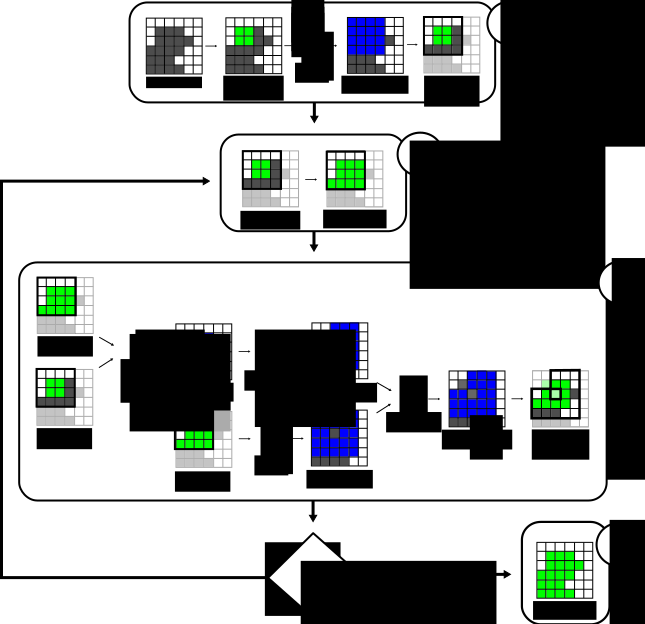
\includegraphics[width=6.7in]{figures/Algorithm.pdf}
\caption{Our algorithm for tracking the active computational domain. Image data is shown in grey, the currently segmented area in the level set field is shown in green, and intermediate results for computing the active computational domain are shown in blue. The active computational domain is outlined in black, and inactive elements are shown as partially transparent. The user places a seed to initialize the level set field and the initial active set is computed according to the spatial derivatives of the level set field (a). During each iteration the level set field is updated at all active elements (b). The new active computational domain is computed according to the temporal and spatial derivatives of the level set field (c). If the new active computational domain is empty (d) then our segmentation has globally converged (e). Otherwise we go to (b).}
}

\begin{document}
\maketitle

\begin{figure}[t]
\centering
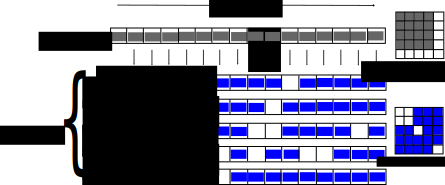
\includegraphics[width=3.3in]{figures/NewActive.pdf}
\caption{Generating new active coordinates. There may be duplicate coordinates in the auxiliary buffers when taken collectively. All duplicate coordinates must subsequently be removed (see Figure~\ref{fig:remove}).}
\label{fig:generate}
\end{figure}

\begin{Listing}[t]
    \caption{Generating new active coordinates. The temporal and spatial derivatives of the level set field are tested on line 5. $m$ is the current size of the active computational domain. \label{pseudo:generate} }
    \begin{algorithmic}[1]
        \FOR { $h \gets 0$ to $m$ in parallel }
            \STATE { $\boldv \gets V_h$ } 
            \STATE { $g \gets \mbox{false}$ }
            \FORALL { coordinates $\boldn \in \nv$ }
                \IF { $ \phiread_{\boldn} \neq \phiwrite_{\boldn} $ \textbf{ and } $ \phiread_{\boldn} \neq \phiread_{\boldv} $ }
                    \STATE { $g \gets \mbox{true}$ }
                    \STATE { $\mathbf{e} \gets \boldn - \boldv$ }
                    \STATE { $B^{\mathbf{e}}_{h} \gets \boldn $ }
                \ENDIF
            \ENDFOR
            \IF { $g$ }
                \STATE { $B^{ \leftbracket 0,0,0 \rightbracket }_{h} \gets \boldv $ }
            \ENDIF                    
        \ENDFOR
    \end{algorithmic}
\end{Listing}

\section{Algorithmic Details}
\label{sec:aWorkEfficientParallelAlgorithm}

%-------------------------------------------------------------------------
\subsection{Assumptions}
\label{subsec:assumptions}

We define the set $ \nx $ to be the set of all elements in the local neighborhood of $\boldx$. We define $m$ to be the current size of the active computational domain. We assume the level set field $ \phi $ is 3D and the elements in $ \phi $ are 6-connected. Therefore it is guaranteed that for all elements $ \boldx \in \domainphi $, $ \nx $ contains at most seven elements: the 6-connected neighbors of $ \boldx $ and $ \boldx $ itself. We define the set $ E = \leftcbracket \leftbracket 0,0,0 \rightbracket , \leftbracket \pm 1,0,0 \rightbracket , \leftbracket 0,\pm 1,0 \rightbracket , \leftbracket 0,0,\pm 1 \rightbracket \rightcbracket $ as the set of offset vectors from a voxel to its 6-connected neighbors.


%-------------------------------------------------------------------------
\subsection{Data Structures and Notation}
\label{subsec:dataStructuresAndNotation}

Our algorithm requires three 3D buffers: $\phiwrite$ and $\phiread$ to store the current and previous level set field respectively; and $U$ to use as a scratchpad. Our algorithm also requires eight 1D buffers: $V$ to store the current dense list of active coordinates; and $B^{ \leftbracket 0,0,0 \rightbracket }$, $B^{ \leftbracket \pm 1,0,0 \rightbracket }$, $B^{ \leftbracket 0, \pm 1,0 \rightbracket }$, and $B^{ \leftbracket 0,0, \pm 1 \rightbracket }$ to use as auxiliary buffers when generating new active coordinates. The size of each buffer is equal to $n = \leftvbracket \mbox{Domain} \leftbracket \phi \rightbracket \rightvbracket$. All buffers are initially filled with null values.

We use a subscript notation to refer to individual buffer elements (e.g. $V_i$ refers to the $i^{th}$ element of $V$; $V_{j \ldots k }$ refers to the range of elements in $V$ from $V_j$ to $V_k$; and $U_{\boldx}$ refers to the element of $U$ with the 3D coordinates $\boldx$).

%We use $V$ to store the current set of active coordinates. We use $\phiread$ and $\phiwrite$ to read from and write to the level set field in a double-buffered fashion. We use $ B^{ \leftbracket 0,0,0 \rightbracket }$, $B^{ \leftbracket 0,0, \pm 1 \rightbracket }$, $B^{ \leftbracket 0, \pm 1,0 \rightbracket }$, and $B^{ \leftbracket \pm 1,0,0 \rightbracket }$ as auxiliary buffers to store intermediate output as we're generating new active coordinates. Finally we use $U$ as a scratchpad buffer. All buffers are initially filled with null values.

%-------------------------------------------------------------------------
\subsection{Generating New Active Coordinates}
\label{subsec:generatingNewActiveCoordinates}

We generate new active coordinates as shown in Figure \ref{fig:generate} and Listing \ref{pseudo:generate}.

%-------------------------------------------------------------------------
\subsection{Removing Duplicate Active Coordinates}
\label{subsec:removingDuplicateActiveCoordinates}

We make the observation that although there may be duplicate coordinates in the seven auxiliary buffers taken collectively, it is guaranteed that there are no duplicate coordinates in each of the seven auxiliary buffers taken individually. This is because there are no duplicate coordinates in $V_{0 \ldots m}$ and for all offset vectors $\mathbf{e} \in E$, either $B^{\mathbf{e}}_{i} = V_i + \mathbf{e} $ or ${B^{\mathbf{e}}_i = \mbox{null}$ for all array indices $i$ where $0 \leq i \leq m$.

Based on the guarantee in the previous paragraph, we are able to remove all duplicate coordinates in seven passes without requiring any additional sorting or synchronization primitives. We describe this process in Listing~\ref{pseudo:5} and Figure~\ref{fig:remove}.

%-------------------------------------------------------------------------
\subsection{Compacting the New Active Coordinates}
\label{subsec:compactingTheNewActiveCoordinates} 

We compact the seven auxiliary buffers in parallel to produce a new dense list of active coordinates and store the result in $V$ as shown in Listing~\ref{pseudo:5}. Since we only ever write to the first $m$ elements of each auxiliary buffer, we only need to compact $7m$ elements in total, rather than compacting the maximum allocated size of each buffer.

After compacting the seven auxiliary buffers, we check if any new active coordinates were compacted into $V$. If so, we clear $B^{\mathbf{e}}_{0 \ldots m}$ for all offset vectors $\mathbf{e} \in E$, update $m$ to be the number of new active coordinates that were compacted into $V$, and go to our next iteration. Otherwise our algorithm has globally converged on the segmented region contained in $\phiread$.

\subsection{Compacting the New Active Coordinates}
\label{subsec:compactingTheNewActiveCoordinates} 

We compact the seven auxiliary buffers in parallel to produce a new dense list of active coordinates and store the result in $V$ as shown in Listing~\ref{pseudo:5}. Since we only ever write to the first $m$ elements of each auxiliary buffer, we only need to compact $7m$ elements in total, rather than compacting the maximum allocated size of each buffer.

After compacting the seven auxiliary buffers, we check if any new active coordinates were compacted into $V$. If so, we clear $B^{\mathbf{e}}_{0 \ldots m}$ for all offset vectors $\mathbf{e} \in E$, update $m$ to be the number of new active coordinates that were compacted into $V$, and go to our next iteration. Otherwise our algorithm has globally converged on the segmented region contained in $\phiread$.

\begin{figure}[t]
\centering
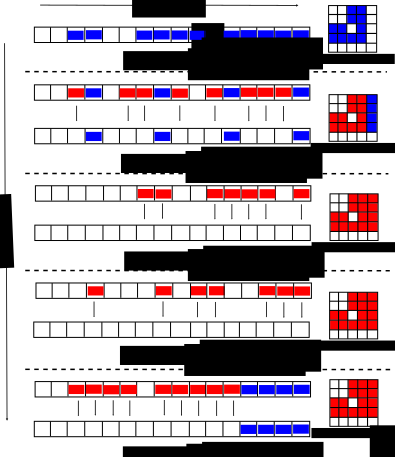
\includegraphics[width=3.3in]{figures/RemoveDuplicates-Alt.pdf}
\caption{Removing duplicate coordinates from the auxiliary buffers in parallel without sorting. Coordinates that have not been previously tagged in the scratchpad buffer are shown in blue. Coordinates that have been previously tagged in the scratchpad buffer are shown in red, and are removed from their containing auxiliary buffer. This process is free of race conditions because each step examines one auxiliary buffer and there are no duplicate coordinates within each auxiliary buffer.}
\label{fig:remove}
\end{figure}
\begin{Listing}[t]
    \caption{Generating a new dense list of unique active coordinates without sorting the auxiliary buffers. $m$ is the current size of the active computational domain. \label{pseudo:5} }
    \begin{algorithmic}[1]
        \STATE { $ E' \gets E - \leftcbracket \leftbracket 0,0,0 \rightbracket , \leftbracket 0,0,1 \rightbracket \rightcbracket $ }
        \FOR { $h \gets 0$ to $m$ in parallel }
            \STATE { $\mathbf{b} \gets B^{ \leftbracket 0,0,0 \rightbracket }_{h}$ }       
            \IF { $ \mathbf{b} \neq \mbox{null}$ }
                \STATE { $ U_{\mathbf{b}} \gets \mbox{tagged}$ }
            \ENDIF
        \ENDFOR                        
        \FORALL { offset vectors $\mathbf{e} \in E' $ } 
            \FOR { $h \gets 0$ to $m$ in parallel }
                \STATE { $\mathbf{b} \gets B^{\mathbf{e}}_{h}$ }            
                \IF { $ \mathbf{b} \neq \mbox{null}$ }
                    \IF { $ U_{\mathbf{b}} = \mbox{tagged} $ }
                        \STATE { $B^{\mathbf{e}}_{h} \gets \mbox{null}$ }
                    \ELSE
                        \STATE { $U_{\mathbf{b}} \gets \mbox{tagged} $ }
                    \ENDIF                                            
                \ENDIF
            \ENDFOR
        \ENDFOR
        \FOR { $h \gets 0$ to $m$ in parallel }
            \STATE { $\mathbf{b} \gets B^{ \leftbracket 0,0,1 \rightbracket }_{h} $ }       
            \IF { $ \mathbf{b} \neq \mbox{null}$ \textbf{ and } $ U_{\mathbf{b}} = \mbox{tagged} $ }
                \STATE { $B^{ \leftbracket 0,0,1 \rightbracket }_{h} \gets \mbox{null}$ }
            \ENDIF
        \ENDFOR                        
        \STATE { $V \gets \mbox{\textbf{compact}} \leftbracket
            B^{ \leftbracket 0,0,0 \rightbracket }_{0 \ldots m},
            B^{ \leftbracket \pm 1, 0, 0 \rightbracket }_{0 \ldots m},
            B^{ \leftbracket 0, \pm 1, 0 \rightbracket }_{0 \ldots m},
            B^{ \leftbracket 0, 0, \pm 1 \rightbracket }_{0 \ldots m} \rightbracket$ }       
    \end{algorithmic}
\end{Listing}    

\begin{figure}[t]
\centering
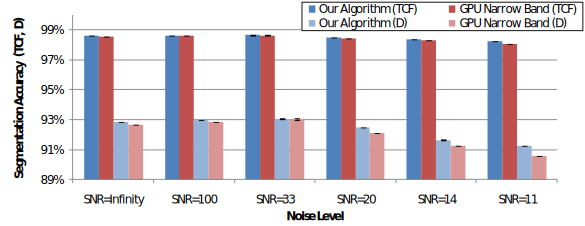
\includegraphics[width=3.3in]{figures/Accuracy.pdf}
\caption{Accuracy of our algorithm and the GPU narrow band algorithm while performing a set of repeated (N=10) white matter segmentations in a $256^3$ head MRI with varying signal-to-noise-ratio (SNR) values. For each segmentation we used a randomly selected seed point and we measured the Dice Coefficient (D) and Total Correct Fraction (TCF). These accuracy measurements are comparable to those reported by Lefohn et al. We speculate the slight difference in accuracy between our algorithm and the GPU narrow band algorithm is due to different floating-point precision semantics in CUDA and OpenGL. }
\label{fig:accuracy}
\end{figure}

\begin{figure}[t]
\centering
\subfigure[]{
\includegraphics[width=3.3in]{figures/SpatialOnly.png}
}
\subfigure[]{
\includegraphics[width=3.3in]{figures/TemporalAndSpatial.png}
}
\caption{The progression of the active computational domain (shown in blue) while segmenting the white matter in a $256^3$ head MRI. In (a) the active computational domain is determined according to the spatial derivative of the level set field. In (b) the active computational domain is determined according to the spatial and temporal derivatives of the level set field. In (b) regions that have locally converged are immediately marked as inactive, resulting in a much smaller active computational domain, and the size of the active computational domain drops to zero when the segmentation has globally converged. }
\label{fig:domaintest}
}
\end{figure}

\section{Evaluation}

We compare the accuracy of our algorithm and the GPU narrow band algorithm in Figure~\ref{fig:accuracy}. We observed that our algorithm was slightly more accurate than the GPU narrow band algorithm with less than 0.2\% variability in all experiments. We speculate that this slight accuracy improvement is due to different floating point precision semantics in CUDA and GLSL. The accuracies we observed are comparable to those reported by Lefohn et al.

In Figure~\ref{fig:domaintest} we qualitatively compare the results of using only the spatial derivatives of the level set field with the results of using both the spatial and temporal derivatives of the level set field to compute the active computational domain.

\end{document}

